\documentclass[a4paper]{article}

% rotate page
\usepackage[landscape, top=1cm, bottom=1.5cm, left=1.5cm, right=1.5cm]{geometry}

\usepackage{graphicx}
\usepackage{subfigure}

\begin{document}
\title{Andrea Ranzato}
% remove date
\date{}
\maketitle

\vspace*{-15mm}
% remove page number on single page
\thispagestyle{empty}

\begin{figure}[!htb]
\centering
\subfigure[]
% Relationship between levels of pollutant and population is nearly linear.
{	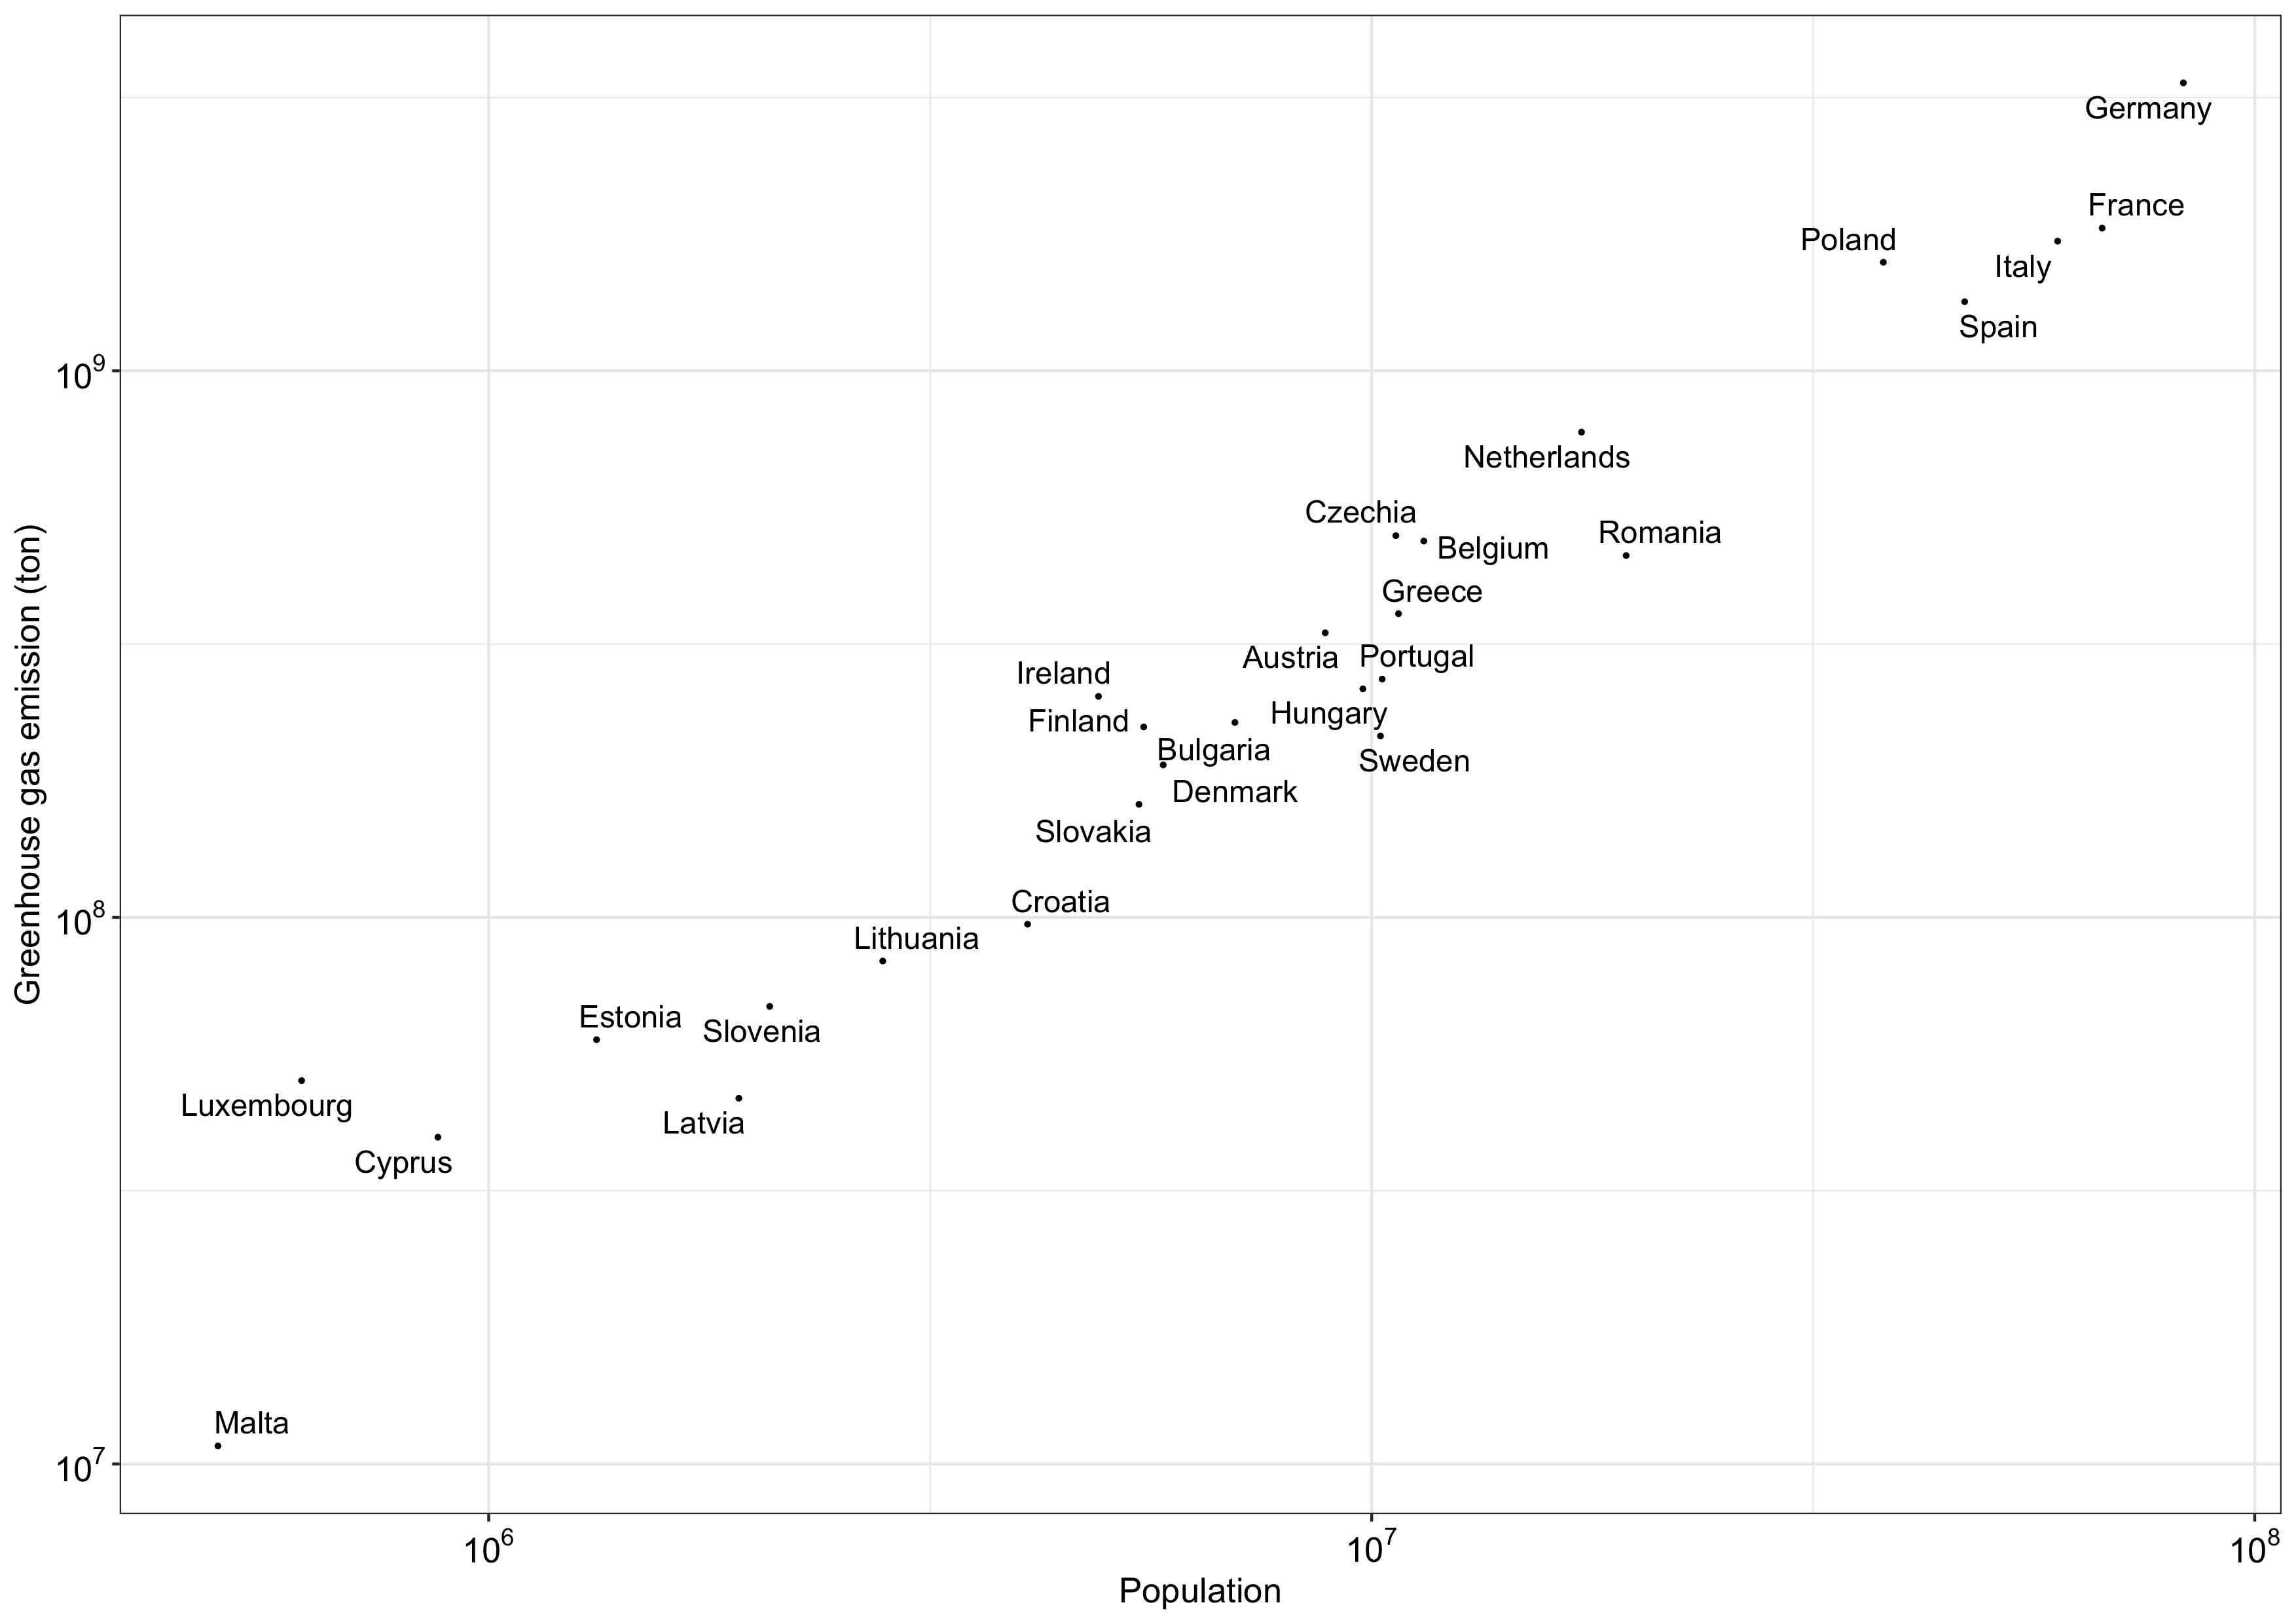
\includegraphics[width=13cm]{plots/population.png}
}\hfill
\subfigure[]
{	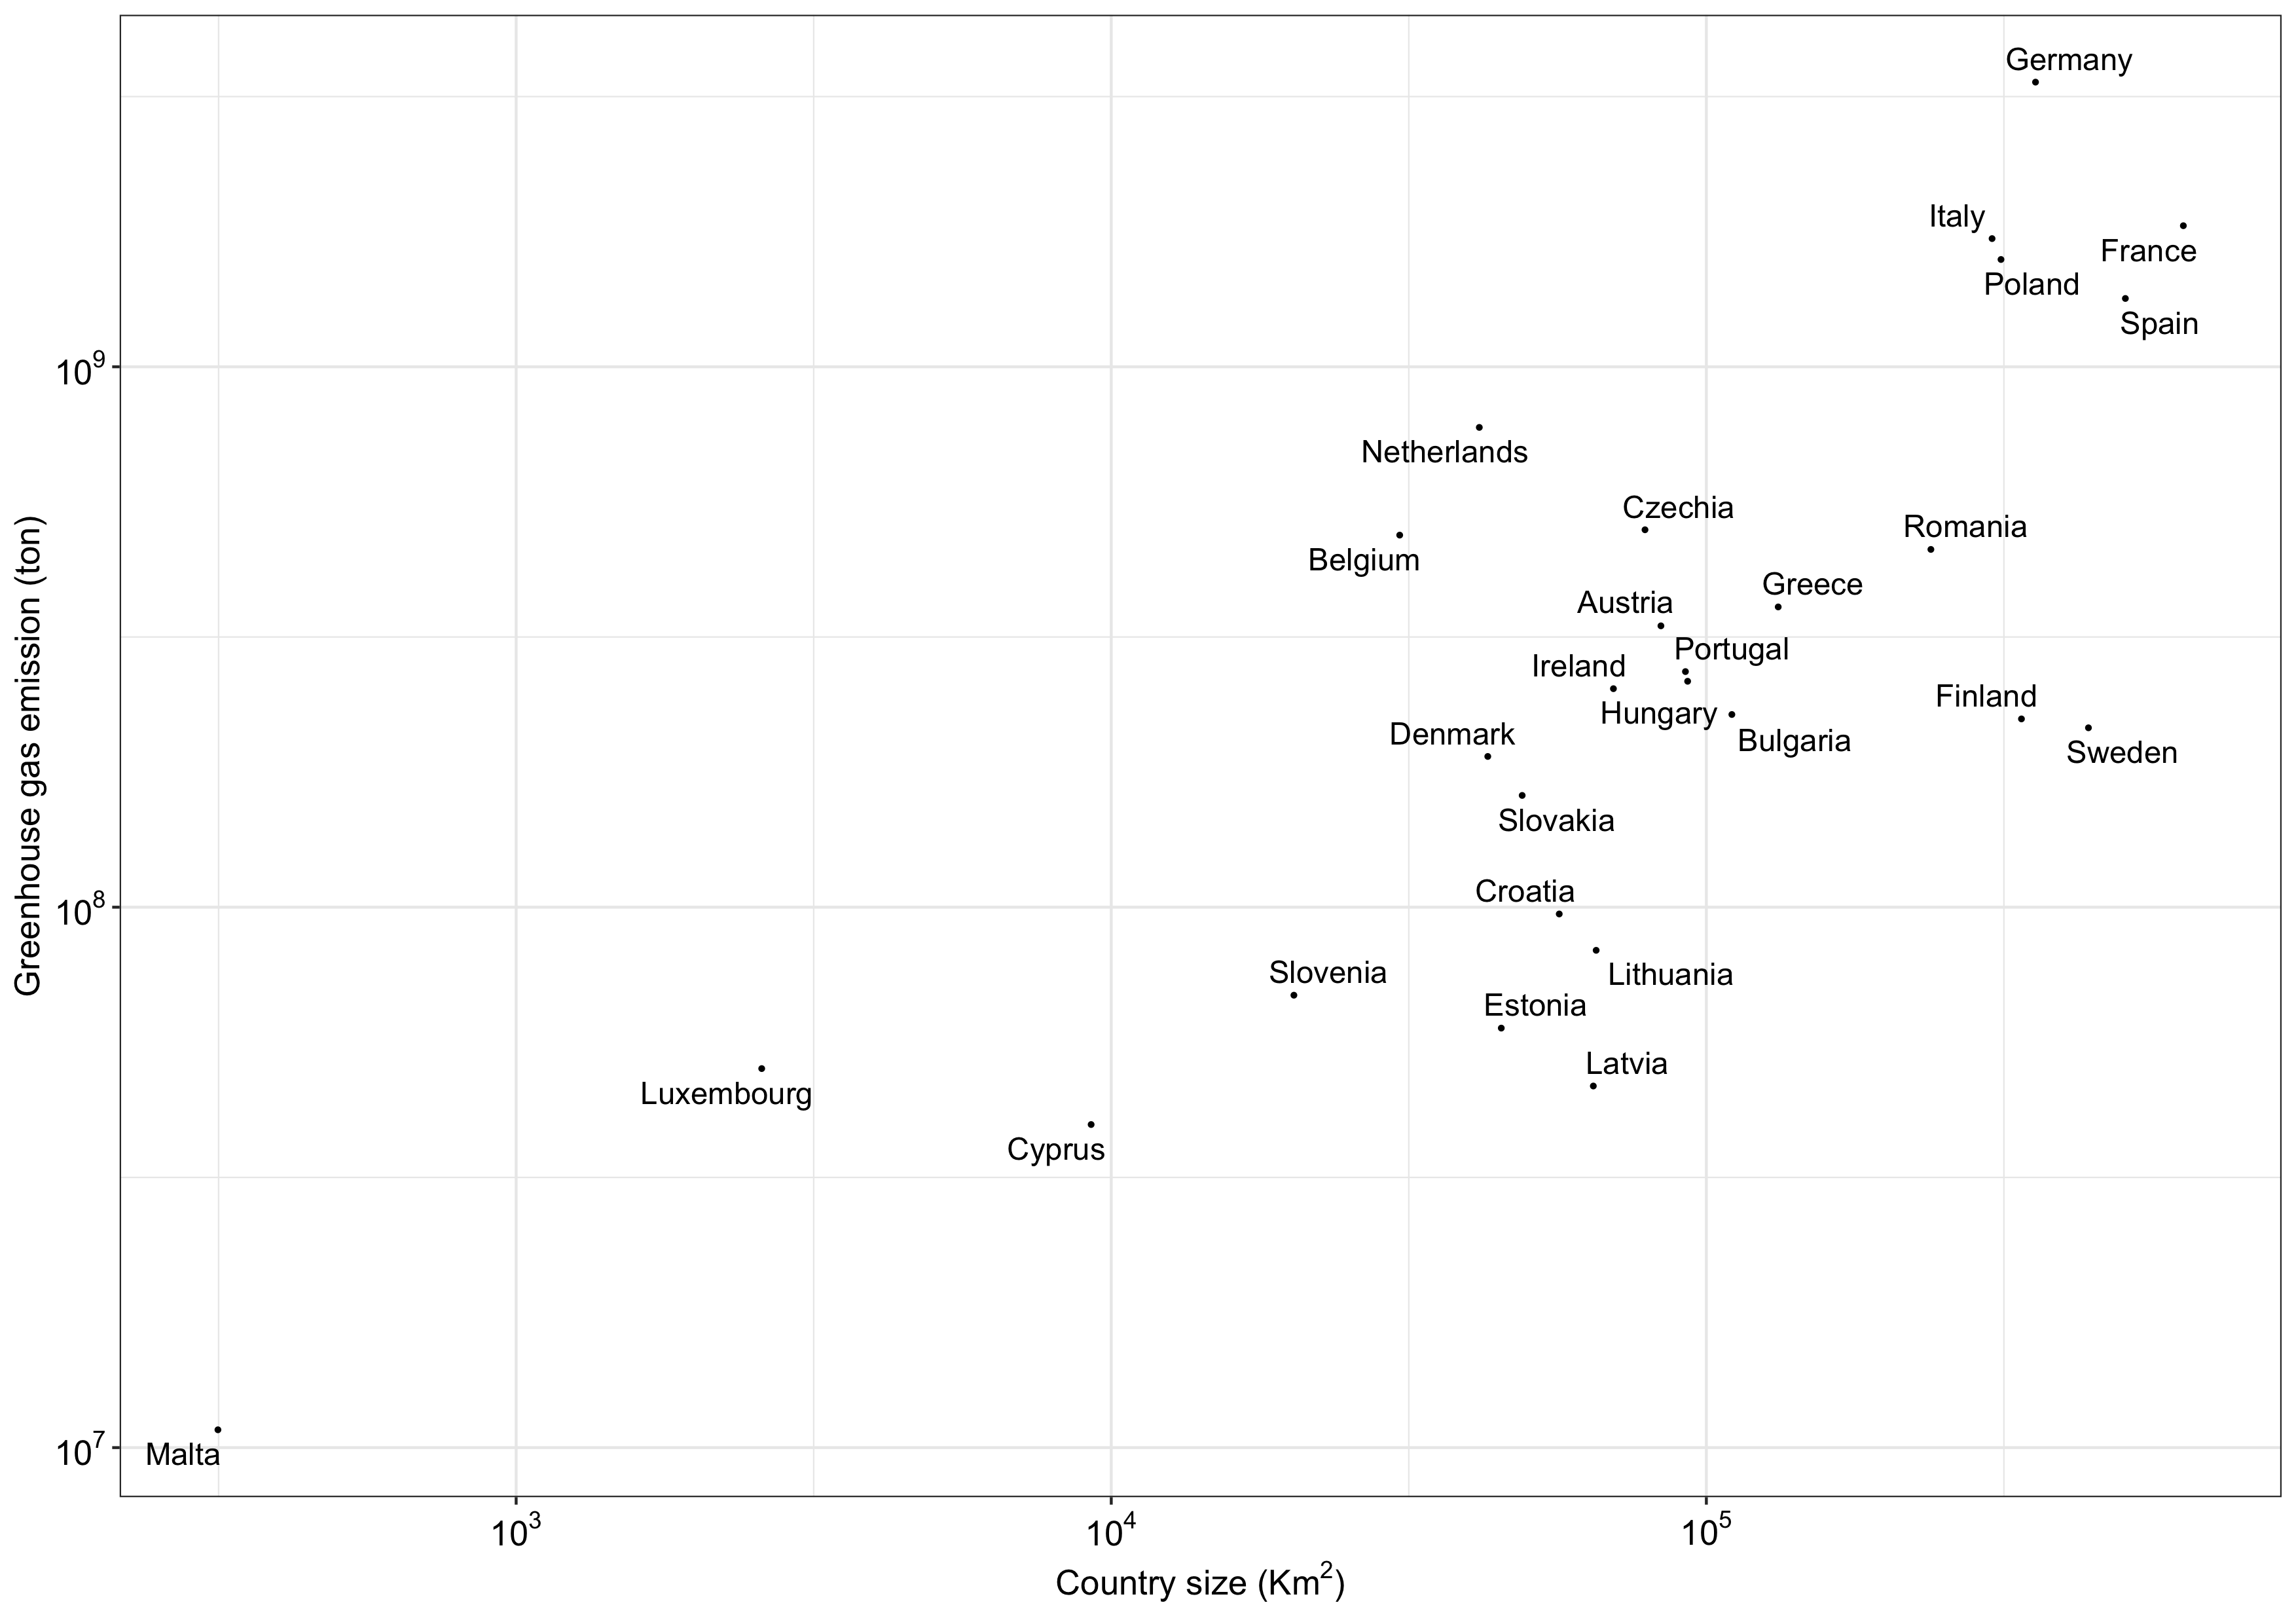
\includegraphics[width=13cm]{plots/dimension.png}
}
\caption{Relation between greenhouse gas emissions, population and country size in the European countries in 2019. Pollutants account for international aviation but not for LULUCF and memory items. Data source: Eurostat.}
\end{figure}

\begin{center}

\begin{itemize}
\item Population is an excellent predictor of greenhouse gas emissions, namely for a given level of population it is associated a low degree of variability in greenhouse gas emissions. 
\item Country size is a weaker predictor of pollutants levels with respect to population. For instance, Holland and Estonia have almost the same size, but the former emits about ten times the amount of pollutants the latter does.
\item Relevant differences in greenhouse gas emissions between countries having the same dimension may be explained with other factors such as, the acquisition of newer technologies, adoption of green policies, etc.

\end{itemize}


\end{center}

\end{document}